\section{Attachements}

\subsection{A1 Tiefpassentwurf mit fir()}
\label{cap:A1}
Mit der Matlab Funktion fir() ist ein FIR-Tiefpassfilter zu entwerfen. Als Defaulteinstellung wird als Fensterfunktion das Hamming-Fenster verwendet. Um die geforderten Grenzwerte einzuhalten muss zunächst die Filterordnung mit dem M\_File Kaiser\_Order\_01.m bestimmt werden. Die Koeffizienten werden mit dem M\_File fir\_1.m gemäß Listing 2 bestimmt. Außerdem wird der Amplitudengang (x=normiert auf Fs/2), das Zeitsignal und der Frequenzgang vor sowie nach dem Filter in einem Diagramm ausgegeben. In den Abbildungen \ref{fig:Attachment_A1_fir_2a_Amplitudengang_PassBand} und \ref{fig:Attachment_A1_fir_2a_Amplitudengang_StopBand} kann gut erkannt werden, das die ripple im Pass- und Stopband eingehalten werden. Die normierten Filterkoeffizienten (normiert auf $\pm$ 1) müssen für die spätere Implementierung in den DSP auf 16-Bit Integer werte angepasst werden. Dazu werden die Koeffizienten mit einem Korrekturfaktor versehen. In Abbildung \ref{lst:fir_2a_matlab} sind die Änderungen von Listing 2 aufgeführt.\\Korrekturwert maximal 1 $\approx$ 32767 $\rightarrow$ 1-Bit Vorzeichen + 15-Bit Wertebereich. 

\begin{equation}
b_{k}(x) = b(x) * 2^{15}-1
\end{equation}

\begin{table}[h]
	\centering
	\begin{tabular}{c | c}
		Parameter	& Wert	\\
		\hline
		Eckfrequenz Durchlassbereich			& $1800~Hz$	\\
		Eckfrequenz Sperrbereich				& $2600~Hz$	\\
		Maximaler Ripple im Durchlassbereich	& $0.5~db$	\\
		Minimale Sperrdämpfung					& $40~db$	\\
		Abtastfrequenz							& $8000~Hz$	\\
	\end{tabular}
\end{table}

\lstinputlisting[style=matlab, caption={fir\_2a.m Matlab-File Auszug - Tiefpassfilter Ordnung 23}, label={lst:fir_2a_matlab}]{Code/fir_2a.m}


\lstinputlisting[style=c, caption={FIR-Filter Koeffizienten Ordnung 23}, label={lst:fir_2a_koeff}]{Code/LP_coeff.h}


\begin{figure}[H]
\centering
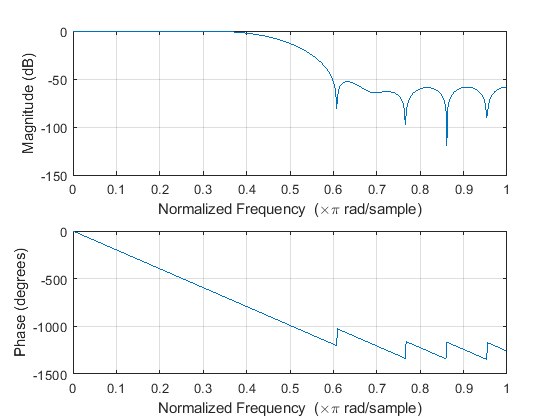
\includegraphics[width=1.0\linewidth]{Bilder/Attachment_A1_fir_2a_Amplitudengang}
\caption{Amplituden und Phasengang - FIR-Filter Tiefpass}
\label{fig:Attachment_A1_fir_2a_Amplitudengang}
\end{figure}


\begin{figure}[H]
\centering
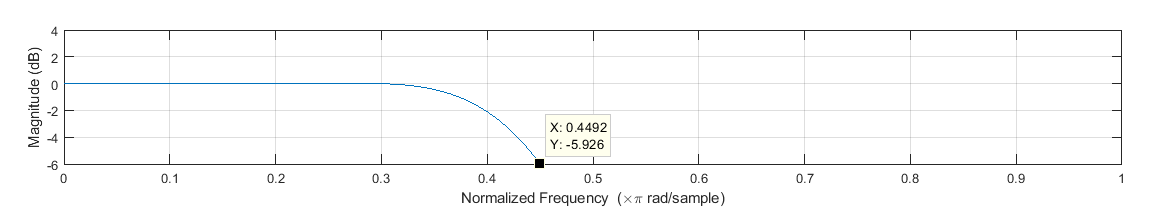
\includegraphics[width=1.0\linewidth]{Bilder/Attachment_A1_fir_2a_Amplitudengang_PassBand}
\caption{Amplitudengang skaliert auf das Passband}
\label{fig:Attachment_A1_fir_2a_Amplitudengang_PassBand}
\end{figure}

\begin{figure}[H]
\centering
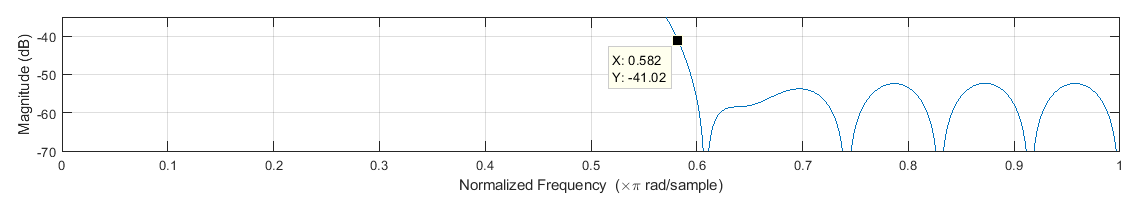
\includegraphics[width=1.0\linewidth]{Bilder/Attachment_A1_fir_2a_Amplitudengang_StopBand}
\caption{Amplitudengang skaliert auf das Stopband}
\label{fig:Attachment_A1_fir_2a_Amplitudengang_StopBand}
\end{figure}

\newpage

\begin{figure}[H]
	\centering
	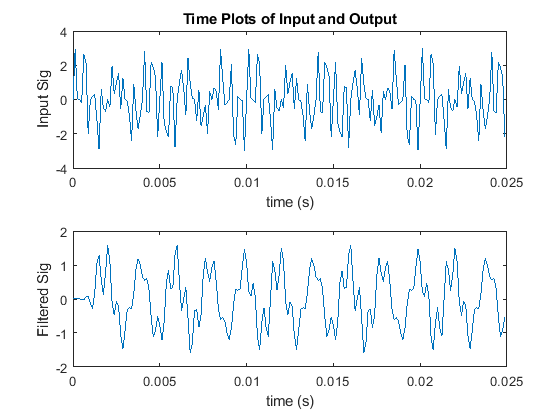
\includegraphics[width=0.8\linewidth]{Bilder/Attachment_A1_fir_2a_Timeplot}
	\caption{Eingangs- und gefiltertes Ausgangszeitsignal  - FIR-Filter Tiefpass}
	\label{fig:Attachment_A1_fir_2a_Timeplot}
\end{figure}

\begin{figure}[H]
	\centering
	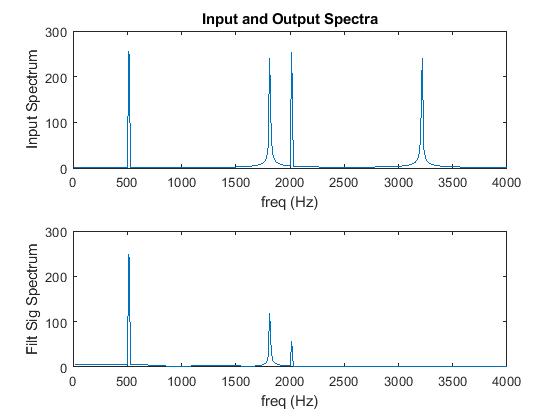
\includegraphics[width=0.8\linewidth]{Bilder/Attachment_A1_fir_2a_Spektrum}
	\caption{Eingangs- gefiltertes Ausgangs Frequenzspektrum}
	\label{fig:Attachment_A1_fir_2a_Spektrum}
\end{figure}

\newpage
\subsection{A2 Tiefpassentwurf mit firpm()}


\noindent Alternativ zur Funktion fir1() soll jetzt die Funktion firpm() verwendet werden um einen FIR-Tiefpassfilter in MATLAB zu entwerfen. In Code-Listing \ref{lst:fir_2b_matlab} sind die Funktionsparameter beschrieben. Die Koeffizienten müssen wie in Kapitel \ref{cap:A1} angepasst werden.

\begin{table}
	\begin{tabular}{c | c}
		Koeffizienten
	\end{tabular}
\end{table}

\lstinputlisting[style=matlab, caption={fir\_2b.m Matlab-File Auszug - Tiefpassfilter Ordnung 16/18}, label={lst:fir_2b_matlab}]{Code/fir_2b.m}

\lstinputlisting[style=c, caption={FIR-Filter Koeffizienten Ordnung 16}, label={lst:fir_2b_koeff}]{Code/LP_coeff_firpm_17K.h}

\noindent Mit der Koeffizientenanzahl, die von der Funktion firpmord zurückgeliefert wird kann die geforderte Sperrdämpfung von 40 db nicht eingehalten werden. Der Amplitudengang ist in Abbildung \ref{fig:Attachment_A2_fir_2b_Amplitudengang_17K}, \ref{fig:Attachment_A2_fir_2b_Amplitudengang_PassBand_17K} und \ref{fig:Attachment_A2_fir_2b_Amplitudengang_StopBand_17K} dargestellt. \textbf{Dieser Zustand ist uns erst in der Versuchsnachbereitung aufgefallen, sodass wir alle folgenden Kapitel mit den Filterkoeffizienten der Filterordnung 16 bearbeitet haben}. In den nachfolgenden Kapiteln werden wir diesen Zustand nicht weiter behandeln.\\
Um die geforderten Parameter dennoch einhalten zu können müsste man die Koeffizienten um 2 erhöhen. Dadurch würde es ein Filtersystem 18 Ordnung ergeben und die in den Abbildungen \ref{fig:Attachment_A2_fir_2b_Amplitudengang_19K}, \ref{fig:Attachment_A2_fir_2b_Amplitudengang_PassBand_19K} und \ref{fig:Attachment_A2_fir_2b_Amplitudengang_StopBand_19K} gezeigten Amplitudenverläufe zeigen.\\
Des weiteren ist zu beobachten, dass die Eckfrequenz des Passbereiches sich auf etwa $\approx$ 2.15 kHz verschoben hat. Die Eckfrequenz des Sperrbereiches allerdings fest auf 2.6 kHz geblieben ist.

\begin{figure}[H]
\centering
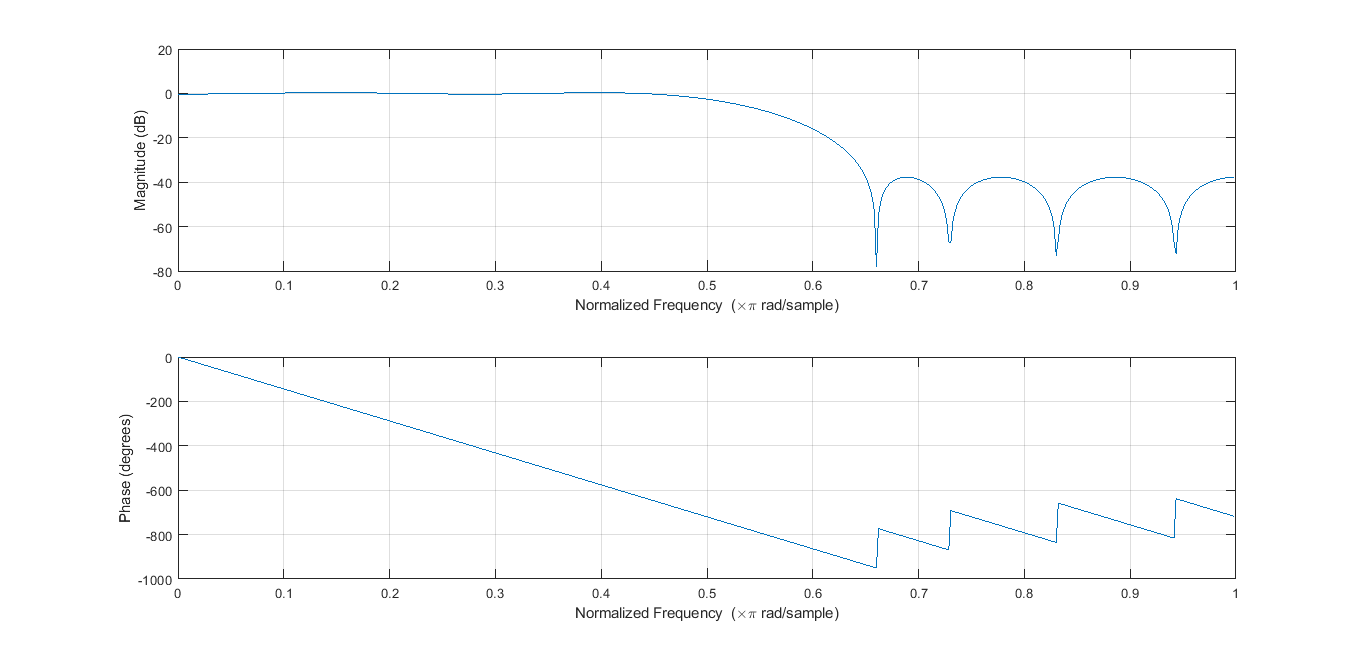
\includegraphics[width=1.0\linewidth]{./Bilder/Attachment_A2_fir_2b_Amplitudengang_17K}
\caption{Amplituden und Phasengang - FIR-Filter Tiefpass - Ordnung: 16}
\label{fig:Attachment_A2_fir_2b_Amplitudengang_17K}
\end{figure}


\begin{figure}[H]
\centering
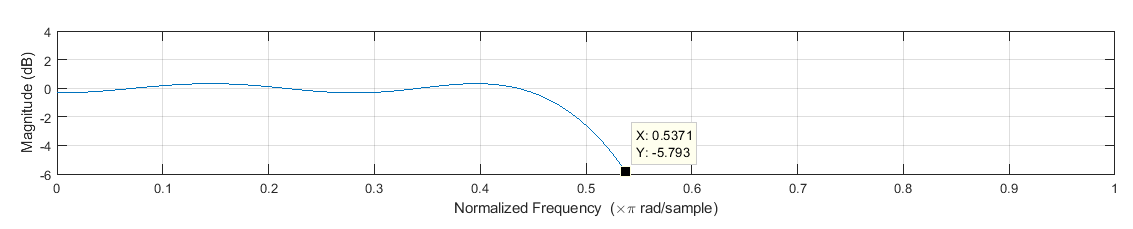
\includegraphics[width=1.0\linewidth]{Bilder/Attachment_A2_fir_2b_Amplitudengang_PassBand_17K}
\caption{Amplitudengang skaliert Passband FIR-Filter Tiefpass - Ordnung: 16}
\label{fig:Attachment_A2_fir_2b_Amplitudengang_PassBand_17K}
\end{figure}

\begin{figure}[H]
\centering
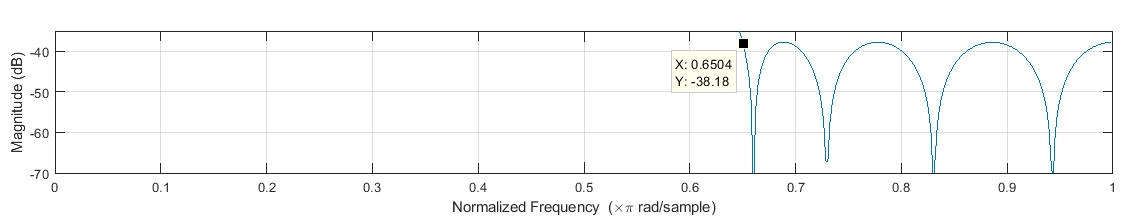
\includegraphics[width=1.0\linewidth]{Bilder/Attachment_A2_fir_2b_Amplitudengang_StopBand_17K}
\caption{Amplitudengang skaliert Stopband FIR-Filter Tiefpass - Ordnung: 16}
\label{fig:Attachment_A2_fir_2b_Amplitudengang_StopBand_17K}
\end{figure}

\newpage


\begin{figure}[H]
	\centering
	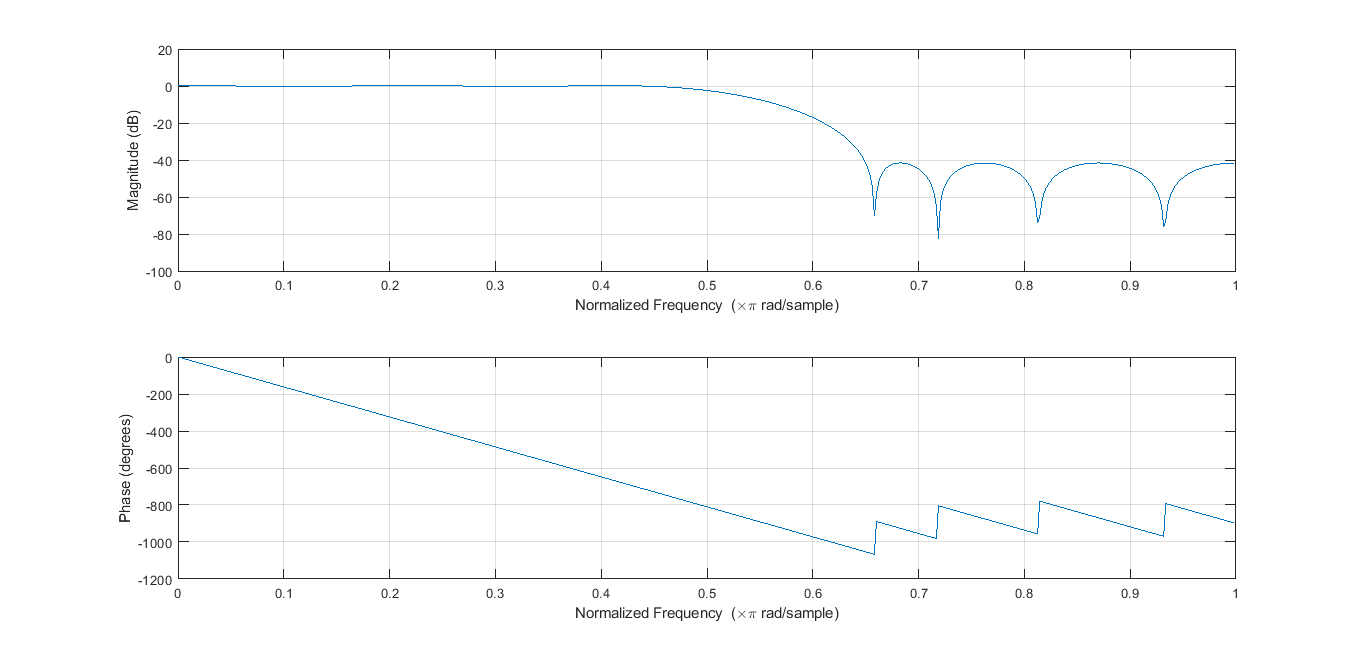
\includegraphics[width=1.0\linewidth]{./Bilder/Attachment_A2_fir_2b_Amplitudengang_19K}
	\caption{Amplituden und Phasengang - FIR-Filter Tiefpass - Ordnung: 18}
	\label{fig:Attachment_A2_fir_2b_Amplitudengang_19K}
\end{figure}


\begin{figure}[H]
	\centering
	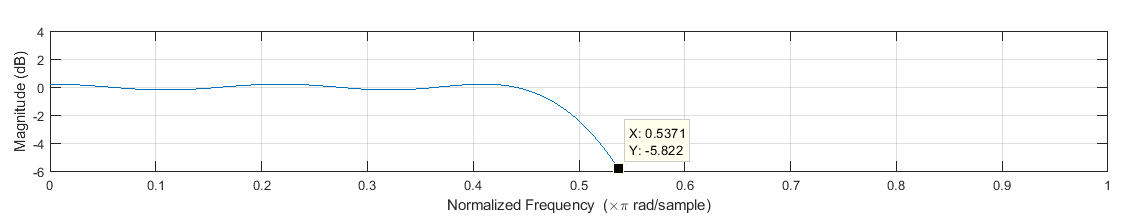
\includegraphics[width=1.0\linewidth]{Bilder/Attachment_A2_fir_2b_Amplitudengang_PassBand_19K}
	\caption{Amplitudengang skaliert Passband FIR-Filter Tiefpass - Ordnung: 18}
	\label{fig:Attachment_A2_fir_2b_Amplitudengang_PassBand_19K}
\end{figure}

\begin{figure}[H]
	\centering
	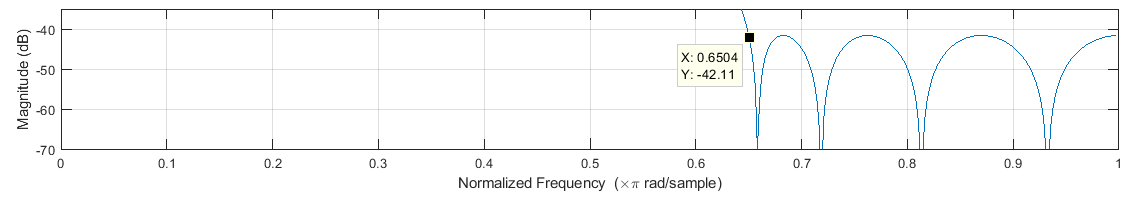
\includegraphics[width=1.0\linewidth]{Bilder/Attachment_A2_fir_2b_Amplitudengang_StopBand_19K}
	\caption{Amplitudengang skaliert Stopband FIR-Filter Tiefpass - Ordnung: 18}
	\label{fig:Attachment_A2_fir_2b_Amplitudengang_StopBand_19K}
\end{figure}

\lstinputlisting[style=c, caption={FIR-Filter Koeffizienten Ordnung 18}, label={lst:fir_2b_koeff}]{Code/LP_coeff_firpm_19K.h}

\newpage


\begin{figure}[H]
\centering
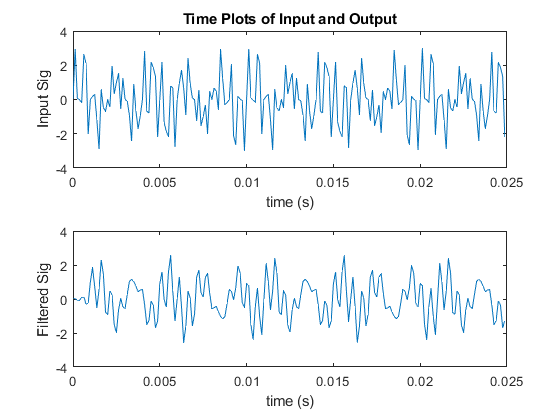
\includegraphics[width=0.85\linewidth]{./Bilder/Attachment_A2_fir_2b_Timeplot}
\caption{Eingangs- und gefiltertes Ausgangszeitsignal  - FIR-Filter Tiefpass}
\label{fig:Attachment_A2_fir_2b_Timeplot}
\end{figure}

\begin{figure}[H]
\centering
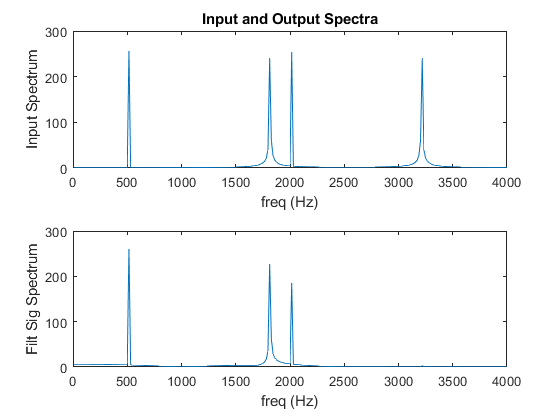
\includegraphics[width=0.85\linewidth]{./Bilder/Attachment_A2_fir_2b_Spektrum}
\caption{Eingangs- gefiltertes Ausgangs Frequenzspektrum}
\label{fig:Attachment_A2_fir_2b_Spektrum}
\end{figure}


\newpage
\subsection{B Bandpass-Filterentwurf}


\lstinputlisting[style=matlab, caption={fir\_3.m Matlab-File Auszug - Bandpassfilter Ordnung 45}, label={lst:fir_3_matlab}]{Code/fir_3.m}

\lstinputlisting[style=c, caption={FIR-Filter Koeffizienten Ordnung 45}, label={lst:fir_3_koeff}]{Code/BP_coeff.h}

\begin{figure}[h]
\centering
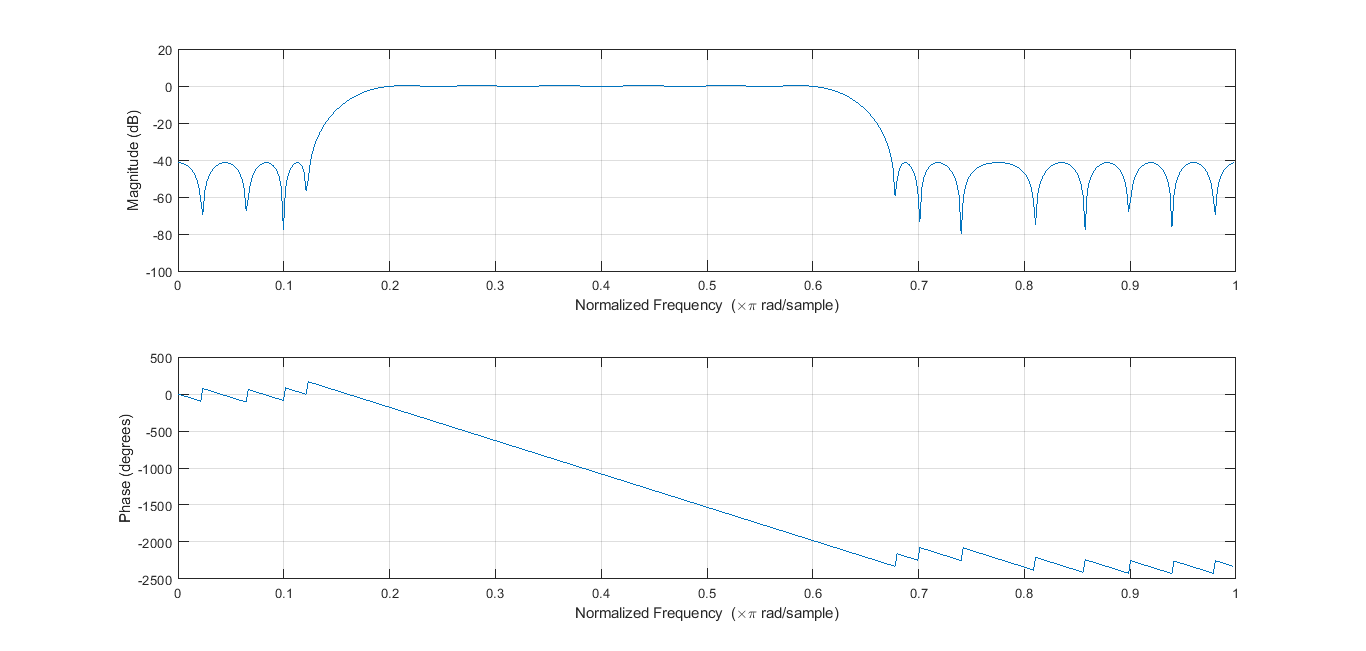
\includegraphics[width=0.7\linewidth]{./Bilder/Attachment_B_fir_3_Amplitudengang}
\caption{Amplituden und Phasengang - FIR-Filter Bandpass}
\label{fig:Attachment_B_fir_3_Amplitudengang}
\end{figure}

\begin{figure}[h]
\centering
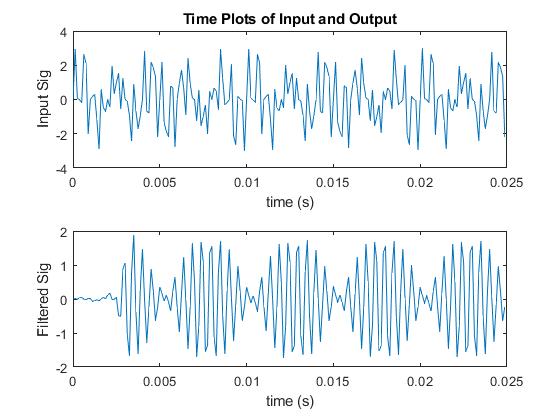
\includegraphics[width=0.7\linewidth]{./Bilder/Attachment_B_fir_3_Timeplot}
\caption{Eingangs- und gefiltertes Ausgangszeitsignal  - FIR-Filter Bandpass}
\label{fig:Attachment_B_fir_3_Timeplot}
\end{figure}


\begin{figure}[h]
\centering
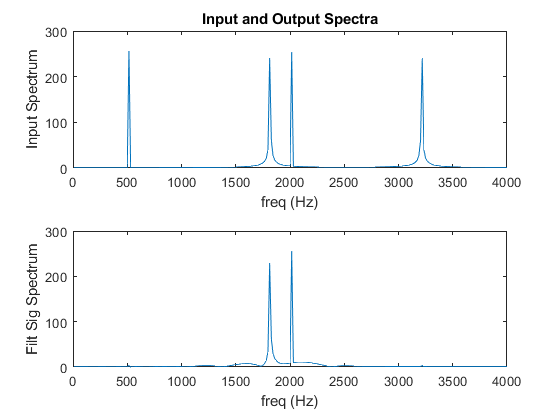
\includegraphics[width=0.7\linewidth]{./Bilder/Attachment_B_fir_3_Spektrum}
\caption{Eingangs- gefiltertes Ausgangs Frequenzspektrum}
\label{fig:Attachment_B_fir_3_Spektrum}
\end{figure}


\newpage
\subsection{C1 Analoge Übertragungscharakteristik des DSK Boards}

\subsection{C2 Echtzeit-Festkomma-Impementierung des FIR-Filters}


\subsection{C3 Vergleich des Amplitudengangs vom FIR-Filter Matlab - DSK Board}

\subsection{D Profiling FIR-ISR}

\subsection{E Weichenfilter Transformation mit $h_{TP} \rightarrow h_{HP} .............$}

\subsection{F Weichenfilter Amplitudengang Hoch- und Tiefpass}

\subsection{G Weichenfilter Transformation mit $h_{TP} \rightarrow h_{HP} ..............$}
 
